\section{det4: the non-amplifying stripes}\label{sec:det4}
\sectionstate{ready}{\texttt{sps\_beam\_test\_26/det4\_sps\_assessment} (scripts 01--17)}
\intent{A production defect seen in the data: 62\,\% of det4's area does not amplify, in stripes. What the data say
about its cause, and why det4's bench numbers are low.}

\tbw{Board map, periodicity, connector and strip-break tests, HV headroom, stability across runs.}
\askStephan{Do the stripes match anything in det4's production (resistive printing, lamination, a particular step)?
Was it seen in QA? Is this paper the place to show it?}
\begin{figure}[t]
  \centering
  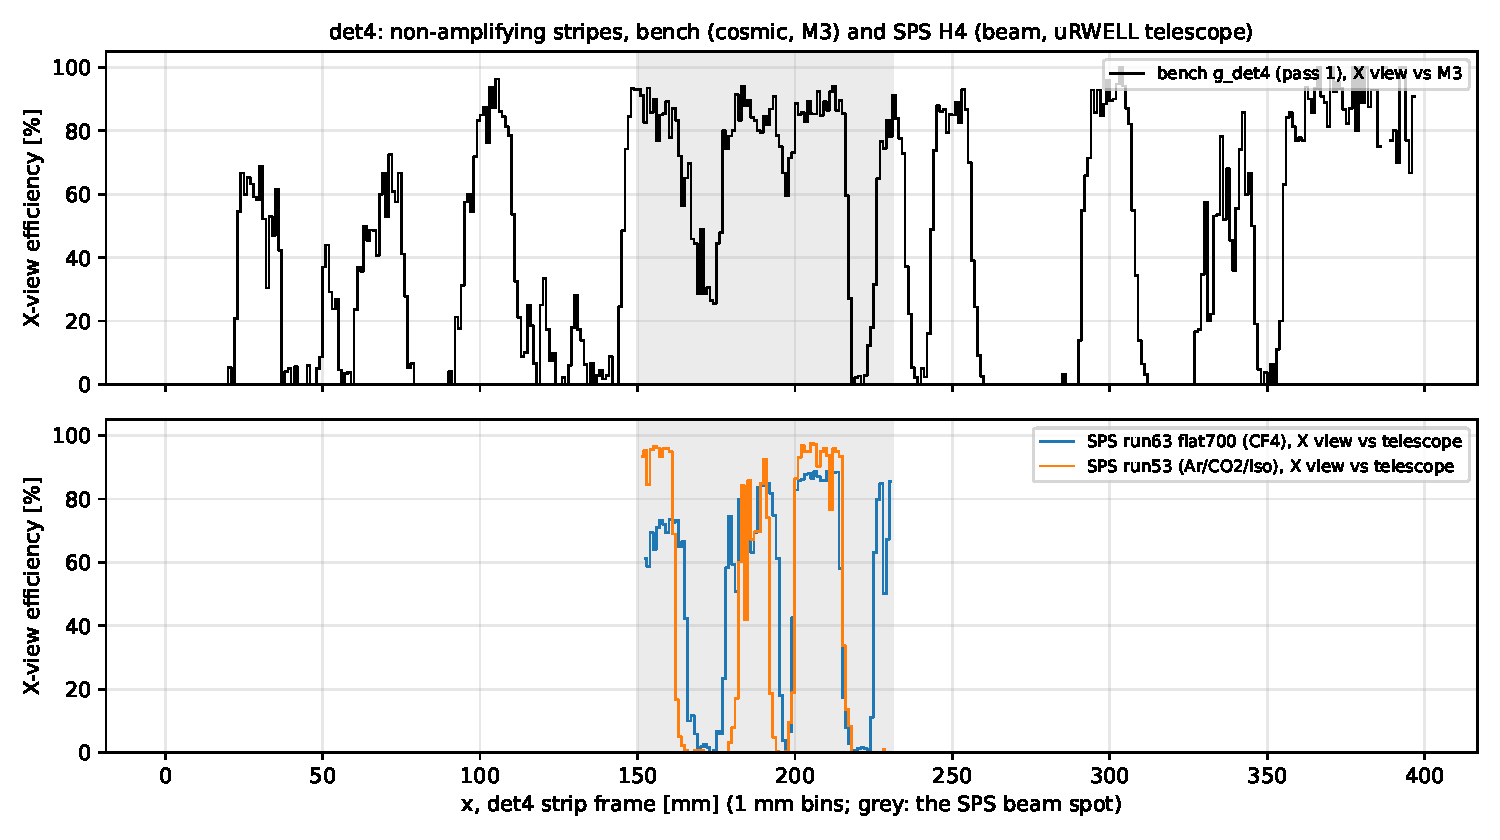
\includegraphics[width=0.75\linewidth]{det4_stripes}
  \caption{\tbw{det4 X-view efficiency across the board (1\,mm bins): top, on the bench against M3; bottom, at SPS against the uRWELL telescope in Ar/CF$_4$/iC$_4$H$_{10}$ (run 63) and Ar/CO$_2$/iC$_4$H$_{10}$ (run 53). Grey band: the SPS beam spot. The same stripes in both.}}
  \label{fig:det4}
\end{figure}
